\hthree{Implementierung}
\label{sec:webcompimp}

\sectionauthor{Julian Kusternigg}

\hfour{Einleitung}

Das Komponentensystem ist der erste Teil der \ZELIA-Frontend-Bibliothek, der entworfen wurde, um den Inhalt der Webseiten darstellen zu können. Der Code im Frontend ist in Typescript (siehe Kapitel TypeScript \ref{sec:TypeScript}, Seite \pageref{sec:TypeScript}) geschrieben, um einen Überblick über die Datentypen zu behalten.

\hfour{Architektur}

Wie bereits im Standard beschrieben, muss es eine Klasse geben, welche von "HTMLElement" erbt, um als "Custom HTML Element" verwendet werden zu können. So gibt es in der \ZELIA\ Implementierung die abstrakte Klasse "Component", von der alle anderen Komponenten erben.

\typescript{code/WebComponents/BaseInterfaces.ts}{Schnittstellen der Basiskomponente}

Die jeweils dazugehörige HTML Quelle wird vom sogenannten "Component Loader", beim Aufruf der Webseite, geladen und zwischengespeichert. Dadurch muss nicht jede Komponente ihren Darstellungscode selbst herunterladen, wie es bei manchen Bibliotheken der Fall ist. Somit ist es kaum merkbar, wenn man eine Seite wechselt. Das Grundgerüst der Seite kann angezeigt werden, während die eigentlichen Informationen noch nachgeladen werden. 

Mit Hilfe von "States" kann man Texte dynamisch ersetzen, wie es auch in anderen Bibliotheken gemacht wird.

\html[code:replhtml]{code/WebComponents/State.html}{Ersetzungsmechanismus (HTML)}

\typescript[code:repljs]{code/WebComponents/State.ts}{Ersetzungsmechanismus (Javascript)}

Dadurch können zum Beispiel nachgeladene Daten eingefügt werden, aber auch die Sprache der Seite kann so geändert werden.

Zusätzlich kann sich das Komponentensystem automatisch Referenzen auf "HTML Elemente" suchen. Dafür muss im Konstruktor der Basiskomponente, von der alle Komponenten erben, nur definiert sein, wie ein Element gefunden wird. Durch den generischen Typen den man der Klasse mitgeben kann, werden die Datentypen der automatisch gefunden Elemente festgelegt (siehe Code \ref{code:kompref}).

\typescript[code:kompref]{code/WebComponents/AutoRef.ts}{Erstellen einer Komponente und suchen einer Referenz}

In diesem Beispiel wird das Element "{\ttfamily button}" gesucht. Dieses Element ist vom Typ "{\ttfamily HTMLButtonElement}" und kann mit "{\ttfamily \#btnInfo}" gefunden werden. Die Raute im Suchfeld besagt, dass der nachfolgende Text die ID von dem HTML-Element ist. Somit würde der Suchtext für das folgende Beispiel zutreffen:

\html{code/WebComponents/IDButton.html}{Beispiel eines HTML Knopfes mit ID}

Im Endeffekt steht dann auf dem Knopf "Click Me". Das "Click" wird mithilfe der
"States" ersetzt und danach wird über die Elementreferenz ein " Me" angehängt. Das automatische Finden von Referenzen ist wichtig, um Events abzufangen oder Elemente zu modifizieren, wenn es notwendig ist.
%TODO: fix all highlighting in code segments 
Wie oben erwähnt, lädt der "Component Loader" die notwendigen HTML-Files und speichert sie. Diese Daten werden dann von der Basis "Component"-Klasse, welche den Namen des HTML-Elements im Konstruktor als Parameter bekommt, verwendet. Über diesen Namen holt sich die Komponente, wenn sie erstellt wird, die HTML Ressource. Wenn sie schließlich angezeigt werden soll, ersetzt sie die "States" und fügt sich selbst in die Webseite hinzu.

\typescript{code/WebComponents/ComponentLoader.ts}{Laden einer Komponente}

Erst nachdem alle Ressourcen der Komponenten geladen wurden, wird der Client-Side-Router (siehe Kapitel Client-Side-Router \ref{sec:csrouter}) erstellt und somit die Seite gestartet. Dadurch kann sichergestellt werden, dass keine verzögerten Ladezeiten durch das Laden der Ressourcen auftreten.

\begin{minipage}{\textwidth}
    \hfour{"Life-Cycle"}
    
    Wenn nun ein eigenes Element erstellt wird, hat der "Loader" die HTML-Ressource bereits geladen. Während der Initialisierung des Elements holt sich dieser die HTML-Ressource als Text. Im Konstruktor der Basiskomponente gibt es neben dem "query"-Parameter, welcher für die automatische Referenzierung verwendet wird, noch die "autoRender"- und "useShadowRoot"-Argumente. Standardmäßig sind beide Werte auf {\ttfamily true} gesetzt. Das heißt, die Komponente wird, sobald sie auf die Seite hinzugefügt wird, ihr HTML anzeigen und in ein "ShadowRoot" eingebunden. Durch das "ShadowRoot" wird es als eigenes Dokument angezeigt, unabhängig von dem wo es eingebunden wird. Dies behebt Überschneidungen von verschieden CSS-Styles. Somit sieht die Komponente jedes Mal gleich aus, unabhängig von der restlichen Seite.
\end{minipage}

Bevor der HTML-Text dargestellt werden kann, werden die "States" ersetzt (siehe Code Beispiel \ref{code:replhtml} und \ref{code:replhtml}, Seite \pageref{code:replhtml}). Danach wird geschaut ob die Elemente, die automatisch referenziert werden sollen, vorhanden sind. Falls sich ein "State" ändert, wird der Inhalt der Komponente automatisch neu erstellt und gerendert. Durch das neu Erstellen der Komponente bekommen auch die referenzierten Elemente neue Referenzen. Das könnte ein Problem sein, wenn man Komponenten hat, bei denen es wichtig ist, dass die Elemente "dieselben" bleiben. Somit sollte man sich um das Modifizieren dieser Komponenten selbst kümmern oder keine "States" ändern, sodass nicht neu gerendert werden muss.

\hfour{Eingebaute Komponenten}

Insgesamt besteht das komplette Frontend aus zwölf Komponenten, die auf acht Seiten verteilt sind (siehe Abbildung \ref{fig:comppageoverview}). Zusätzlich gibt es die "Debug"-Komponente, die vor allem während der Entwicklung praktisch ist, um auf Mobilgeräten die Hintergrundaufgaben mitverfolgen zu können.

\begin{figure}[H]
    \centering
    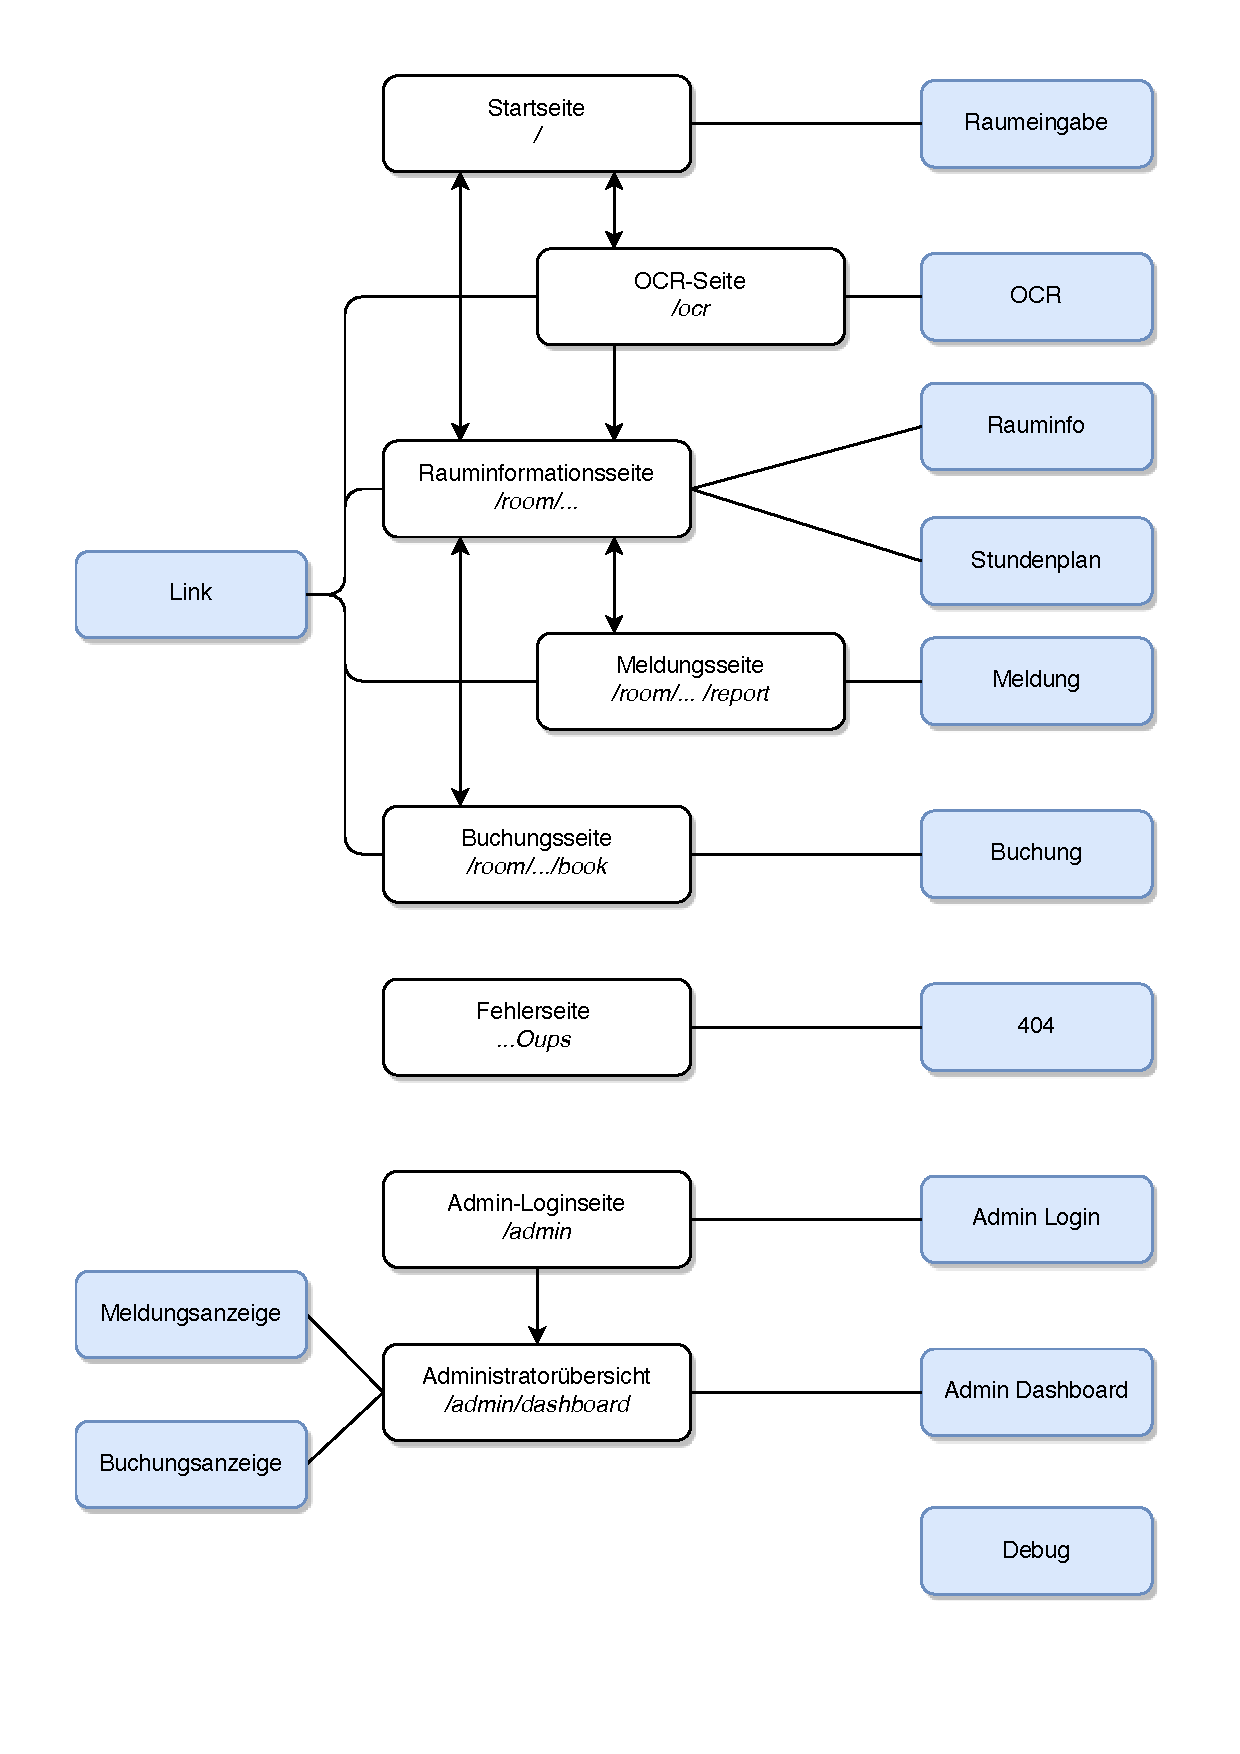
\includegraphics[width=150mm]{media/WebComponents/overview.svg.pdf}
    \caption{Übersicht über alle Komponenten (blau) und Seiten (weiß)}
    \label{fig:comppageoverview}
\end{figure}

\begin{minipage}{\textwidth}
    \hfive{Die Startseite}
    \label{sec:webcompstart}
    
    Auf dem Root-Pfad ("/") liegt die Willkommensseite von \ZELIA. Auf ihr findet man die Raumeingabekomponente, die von der \ZELIA-API alle möglichen Raumnummern abfragt und als Auswahlhilfe anzeigt. Auf Mobilgeräten, wie Smartphones oder Tablets, wird zusätzlich ein Knopf angezeigt. Dieser ermöglicht es die Raumnummer mit der Kamera des Geräts einzulesen. Wenn man auf diesen Knopf drückt, wird man zur "OCR"-Seite weitergeleitet. Gibt man die Raumnummer selbst ein, landet man sofort auf der Rauminformationsseite. Während der manuellen Eingabe werden alle bekannten Räume in einer dynamisch generierten Dropdown-Liste, unter der Eingabebox, angezeigt. Gibt man einen Buchstaben des Raumnamens oder Raumnummer an, so werden nur mehr Ergebnisse angezeigt, in denen das angegebene Muster vorkommt.
\end{minipage}

Beispiel:

\begin{figure}[H]
    \centering
    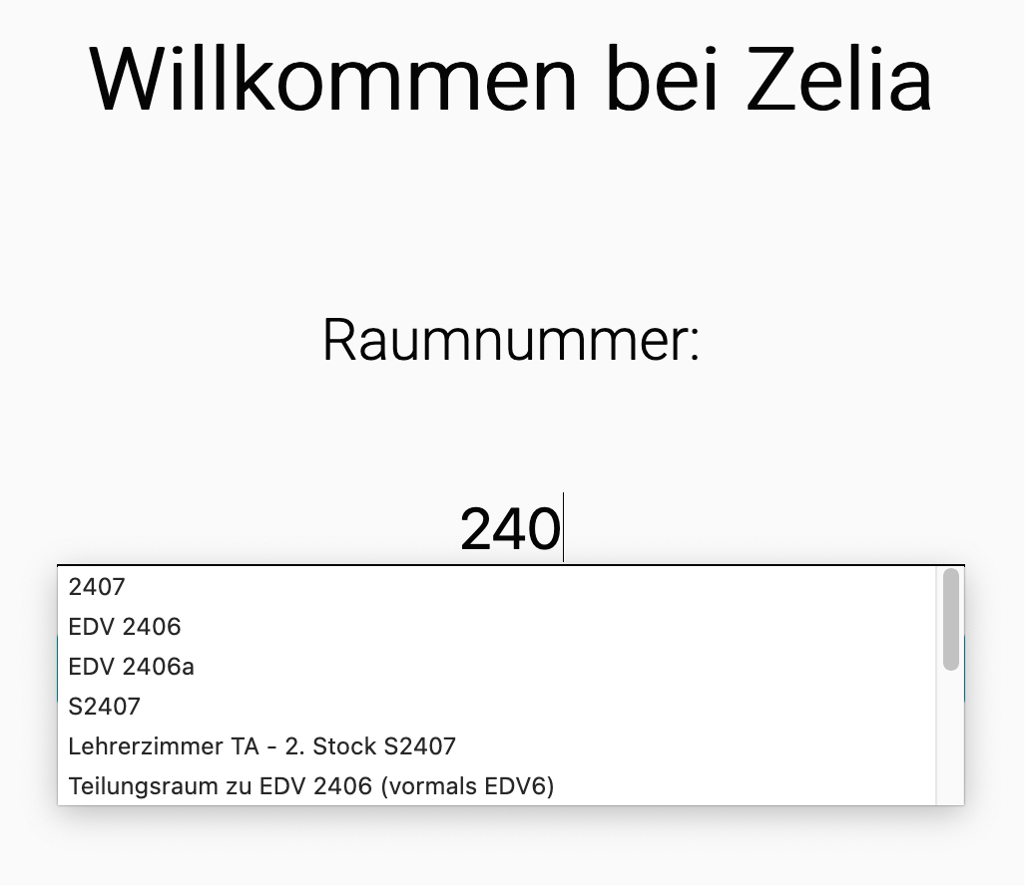
\includegraphics[width=80mm]{media/WebComponents/Startseite_light.png}
    \caption{Startseite}
    \label{fig:compinput}
\end{figure}


\hfive{Die "OCR"-Seite}

Auf dieser Seite können alle Geräte die eine Kamera haben, eine Raumnummer von Raumschildern, Plakaten, usw., einscannen. Diese Anforderung wurde mittels "Optical Character Recognition", kurz "OCR", bewerkstelligt (siehe Kapitel "Optical Character Recognition" \ref{sec:ocr}). Die "OCR"-Seite besteht aus zwei Komponenten. Eine zeigt an was die Kamera sieht und die Andere dient als Link, um zurück zur Startseite zu kommen. Die Komponente, welche den Scanner anzeigt, ist auch zuständig den OCR-Service (siehe Kapitel Tesseract \ref{sec:tesseract}, Seite \pageref{sec:tesseract}) zu starten. Mit Hilfe von diesem wird dann der Text aus den Bildern ausgelesen. Bevor das Bild an den OCR-Service übergeht, wird es durch unsere App auf zwei Farben komprimiert und zusammengeschnitten, sodass nur mehr der markierte Fokusbereich der Kamera weiter zu verarbeiten bleibt (siehe Abbildung \ref{fig:ocrpage}).

\begin{figure}[H]
    \centering
    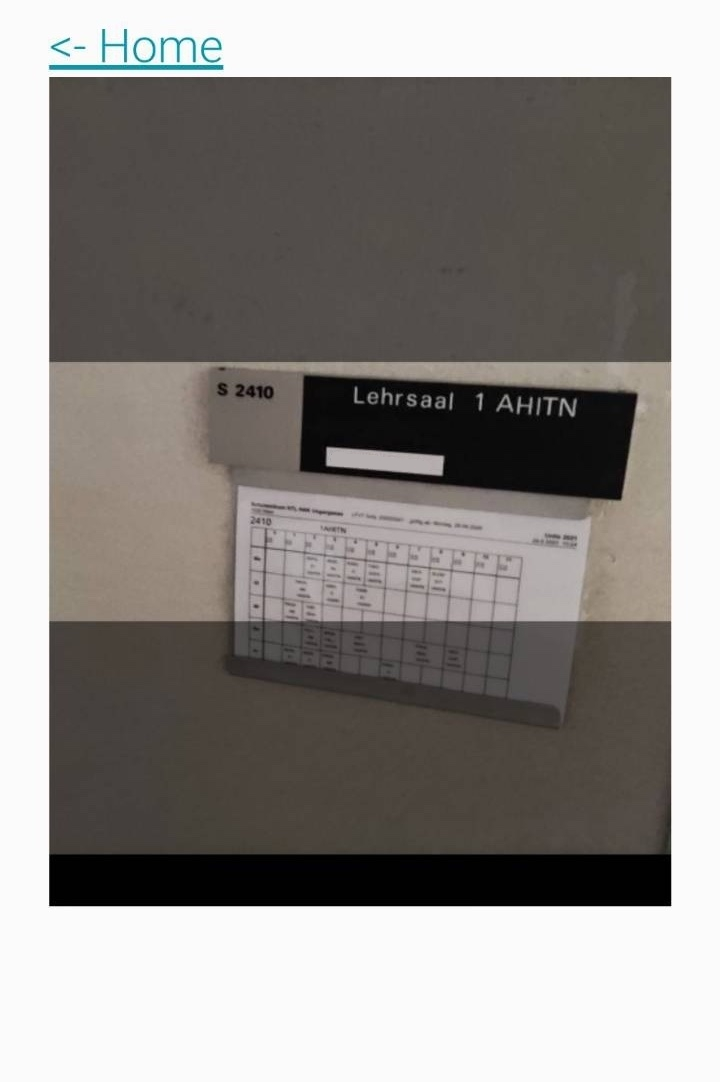
\includegraphics[width=80mm]{media/WebComponents/OCRSeite_light.jpg}
    \caption{OCR-Seite}
    \label{fig:ocrpage}
\end{figure}


Meist liefert der OCR-Prozess eindeutige Ergebnisse. Allerdings kann es auch passieren, gerade wenn viele helle und dunkle Flecken im Hintergrund des Bildes sind, dass diese als Zeichen erkannt werden. Somit ist es notwendig, dass nachdem das Bild in Text umgewandelt wurde, mittels "Regular Expressions" der wichtige Teil aus dem Text herausgefiltert wird. Dieser gesamte Prozess, der Bilder in Text umwandelt, wird mit den Standardwerten einmal pro Sekunde durchgeführt. Dieses Intervall kann einfach verändert werden. Im Fall von \ZELIA ist es standardmäßig eine Sekunde, da dies völlig ausreichend ist, um schnell Raumnummern zu erfassen. Wenn dieses Intervall kleiner werden würde, also wenn mehrmals pro Sekunde Bild zu Text verarbeitet wird, dann könnten schwächere Smartphones schnell warm werden und mehr Energie verbrauchen. Mehr zu OCR und den Messungen der Implementierung später (siehe Kapitel "Optical Character Recognition" \ref{sec:ocr} und Messungen der OCR Implementierung \ref{sec:ocrmessung}, Seite \pageref{sec:ocr} und \pageref{sec:ocrmessung}). Wenn eine Raumnummer erfolgreich eingelesen wurde, wird man automatisch auf die Rauminformationsseite weitergeleitet.

\hfive{Rauminformationsseite}

Wie der Name schon vermuten lässt, kann man auf der Rauminformationsseite alle Daten über einen Raum auslesen. Nachdem man einen Raum, entweder durch manuelle Eingabe oder durch das Einscannen der Nummer ausgewählt hat, wird man auf die jeweilige Rauminformationsseite umgeleitet. Aufgebaut ist die Seite aus insgesamt fünf Komponenten (siehe Abbildung \ref{fig:roominfoframes}). So wie bei der OCR-Seite gibt es auch hier einen Link, welcher zurück auf die Startseite führt. Zwei weitere Komponenten dienen als Knöpfe, um eine Meldung oder Buchung zu einem Raum zu erstellen. Wenn man einen der beiden drückt, wird man auf die jeweilige Seite, Meldung oder Buchung umgeleitet. Die letzten zwei Komponenten auf dieser Seite sind die interessantesten, denn sie zeigen die Informationen zu einem Raum an. Die eine Komponente zeigt eine aufklappbare Liste an, um die physikalischen Daten eines Raumes anzusehen. Die andere Komponente wird verwendet, um den jeweiligen Raumstundenplan dazustellen.

\begin{figure}[H]
    \centering
    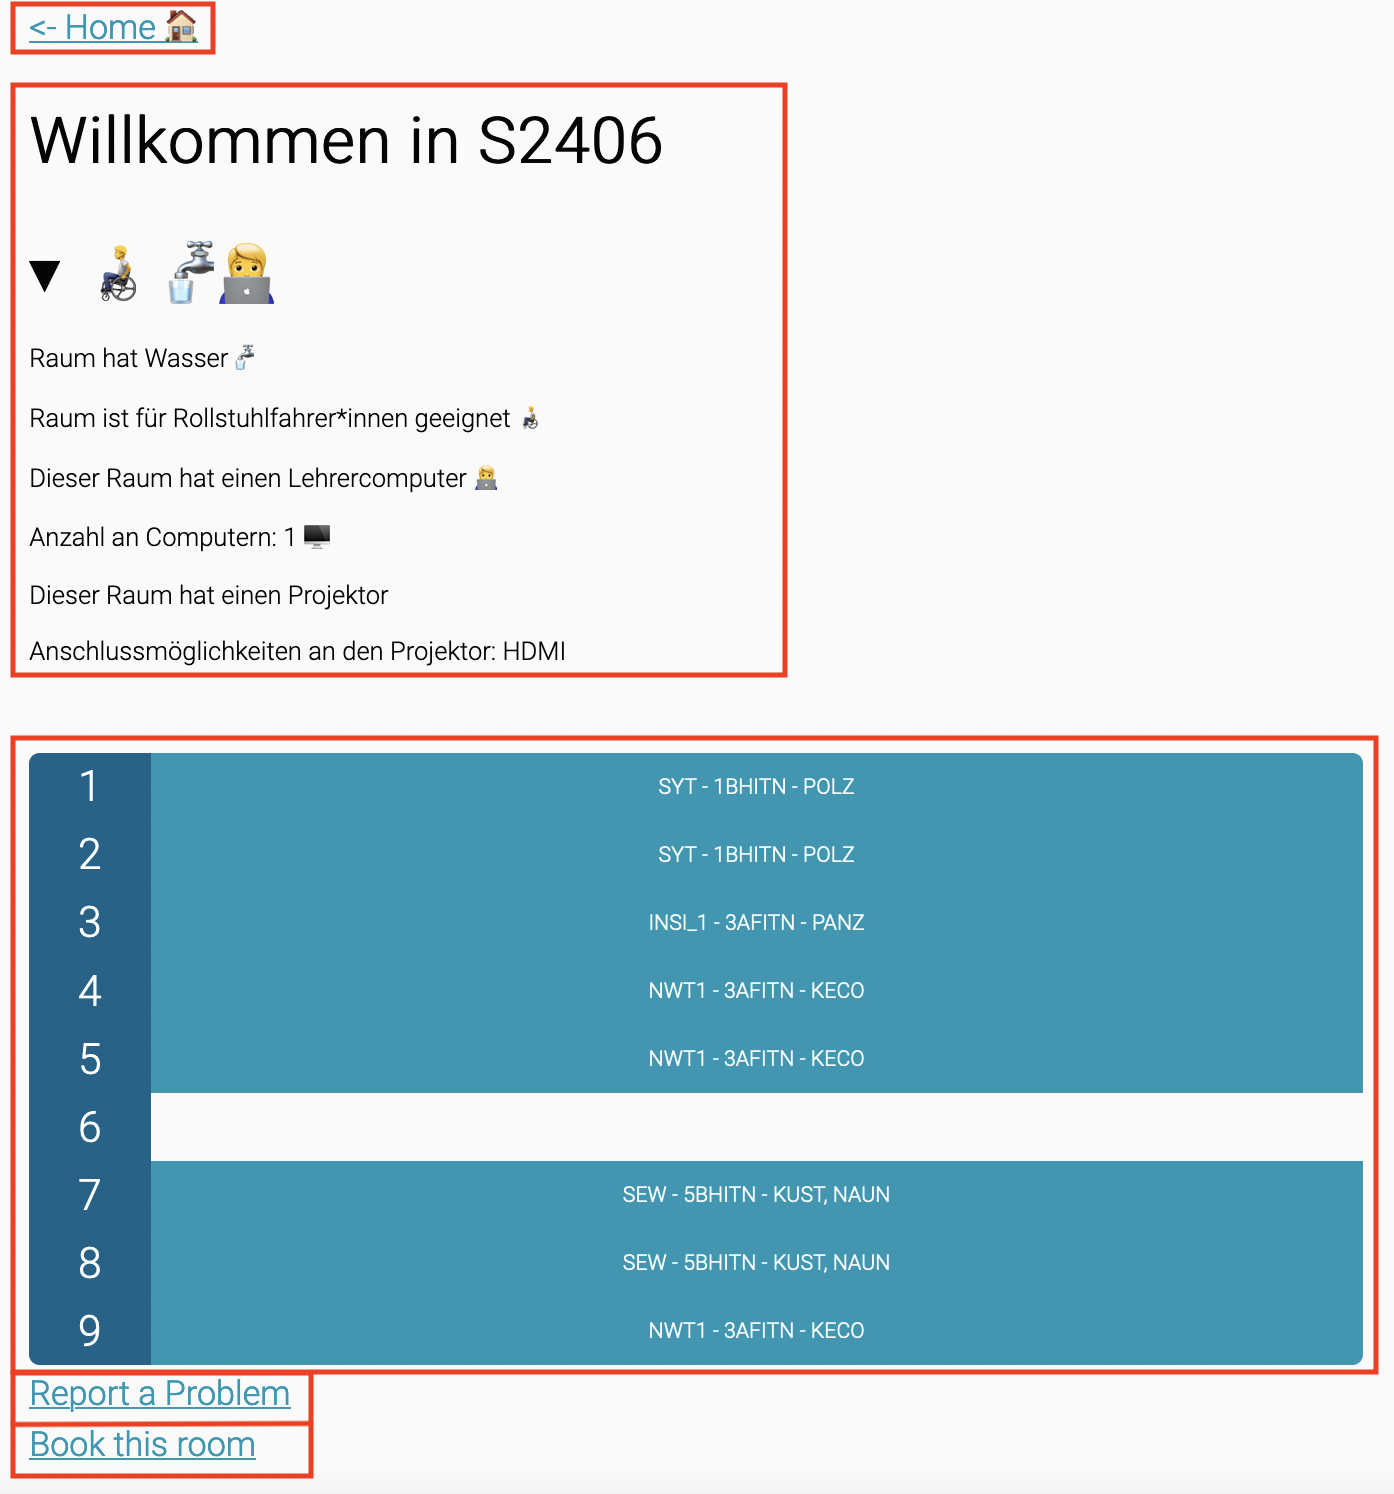
\includegraphics[width=120mm]{media/WebComponents/Rauminformationsseite_frames.png}
    \caption{Rauminformationsseite}
    \label{fig:roominfoframes}
\end{figure}

\hfive{Meldungen und Buchungen}

Die Meldungs- und Buchungsseite sind zwei verschiedene Seiten, welche allerdings ähnlich aufgebaut sind. Erreichen kann man sie nur über die Rauminformationsseite, da sie sich auf einen bestimmten Raum beziehen. Dadurch, dass sie zwei verschiedene Aufgaben haben, werden sie getrennt behandelt und nicht auf einer Seite zusammengefasst. Beide Seiten bestehen aus zwei Komponenten:
\begin{itemize}
    \item Einem Formular, zur Beschreibung und Angabe der Daten
    \item Einem Link, welcher zurück zur Rauminformationsseite führt
\end{itemize}

Damit man Defekte in einem Raum melden kann, gibt man eine EDU-Mail-Adresse, das Datum sowie Uhrzeit wann der Defekt das erste Mal aufgetreten ist und eine Beschreibung des Problems an. Wie schon erläutert, wird die Mail-Adresse verwendet, um Schüler*innen identifizieren zu können, ohne dass sie sich einen Account anlegen müssen. Nach Absenden des Formulars bekommt man einen Bestätigungslink auf die angegebene Mail-Adresse, um die Meldung zu bestätigen. So ist das Meldesystem nicht anonym und dadurch können Falsch-Meldungen verringert werden.

\begin{figure}[H]
    \centering
    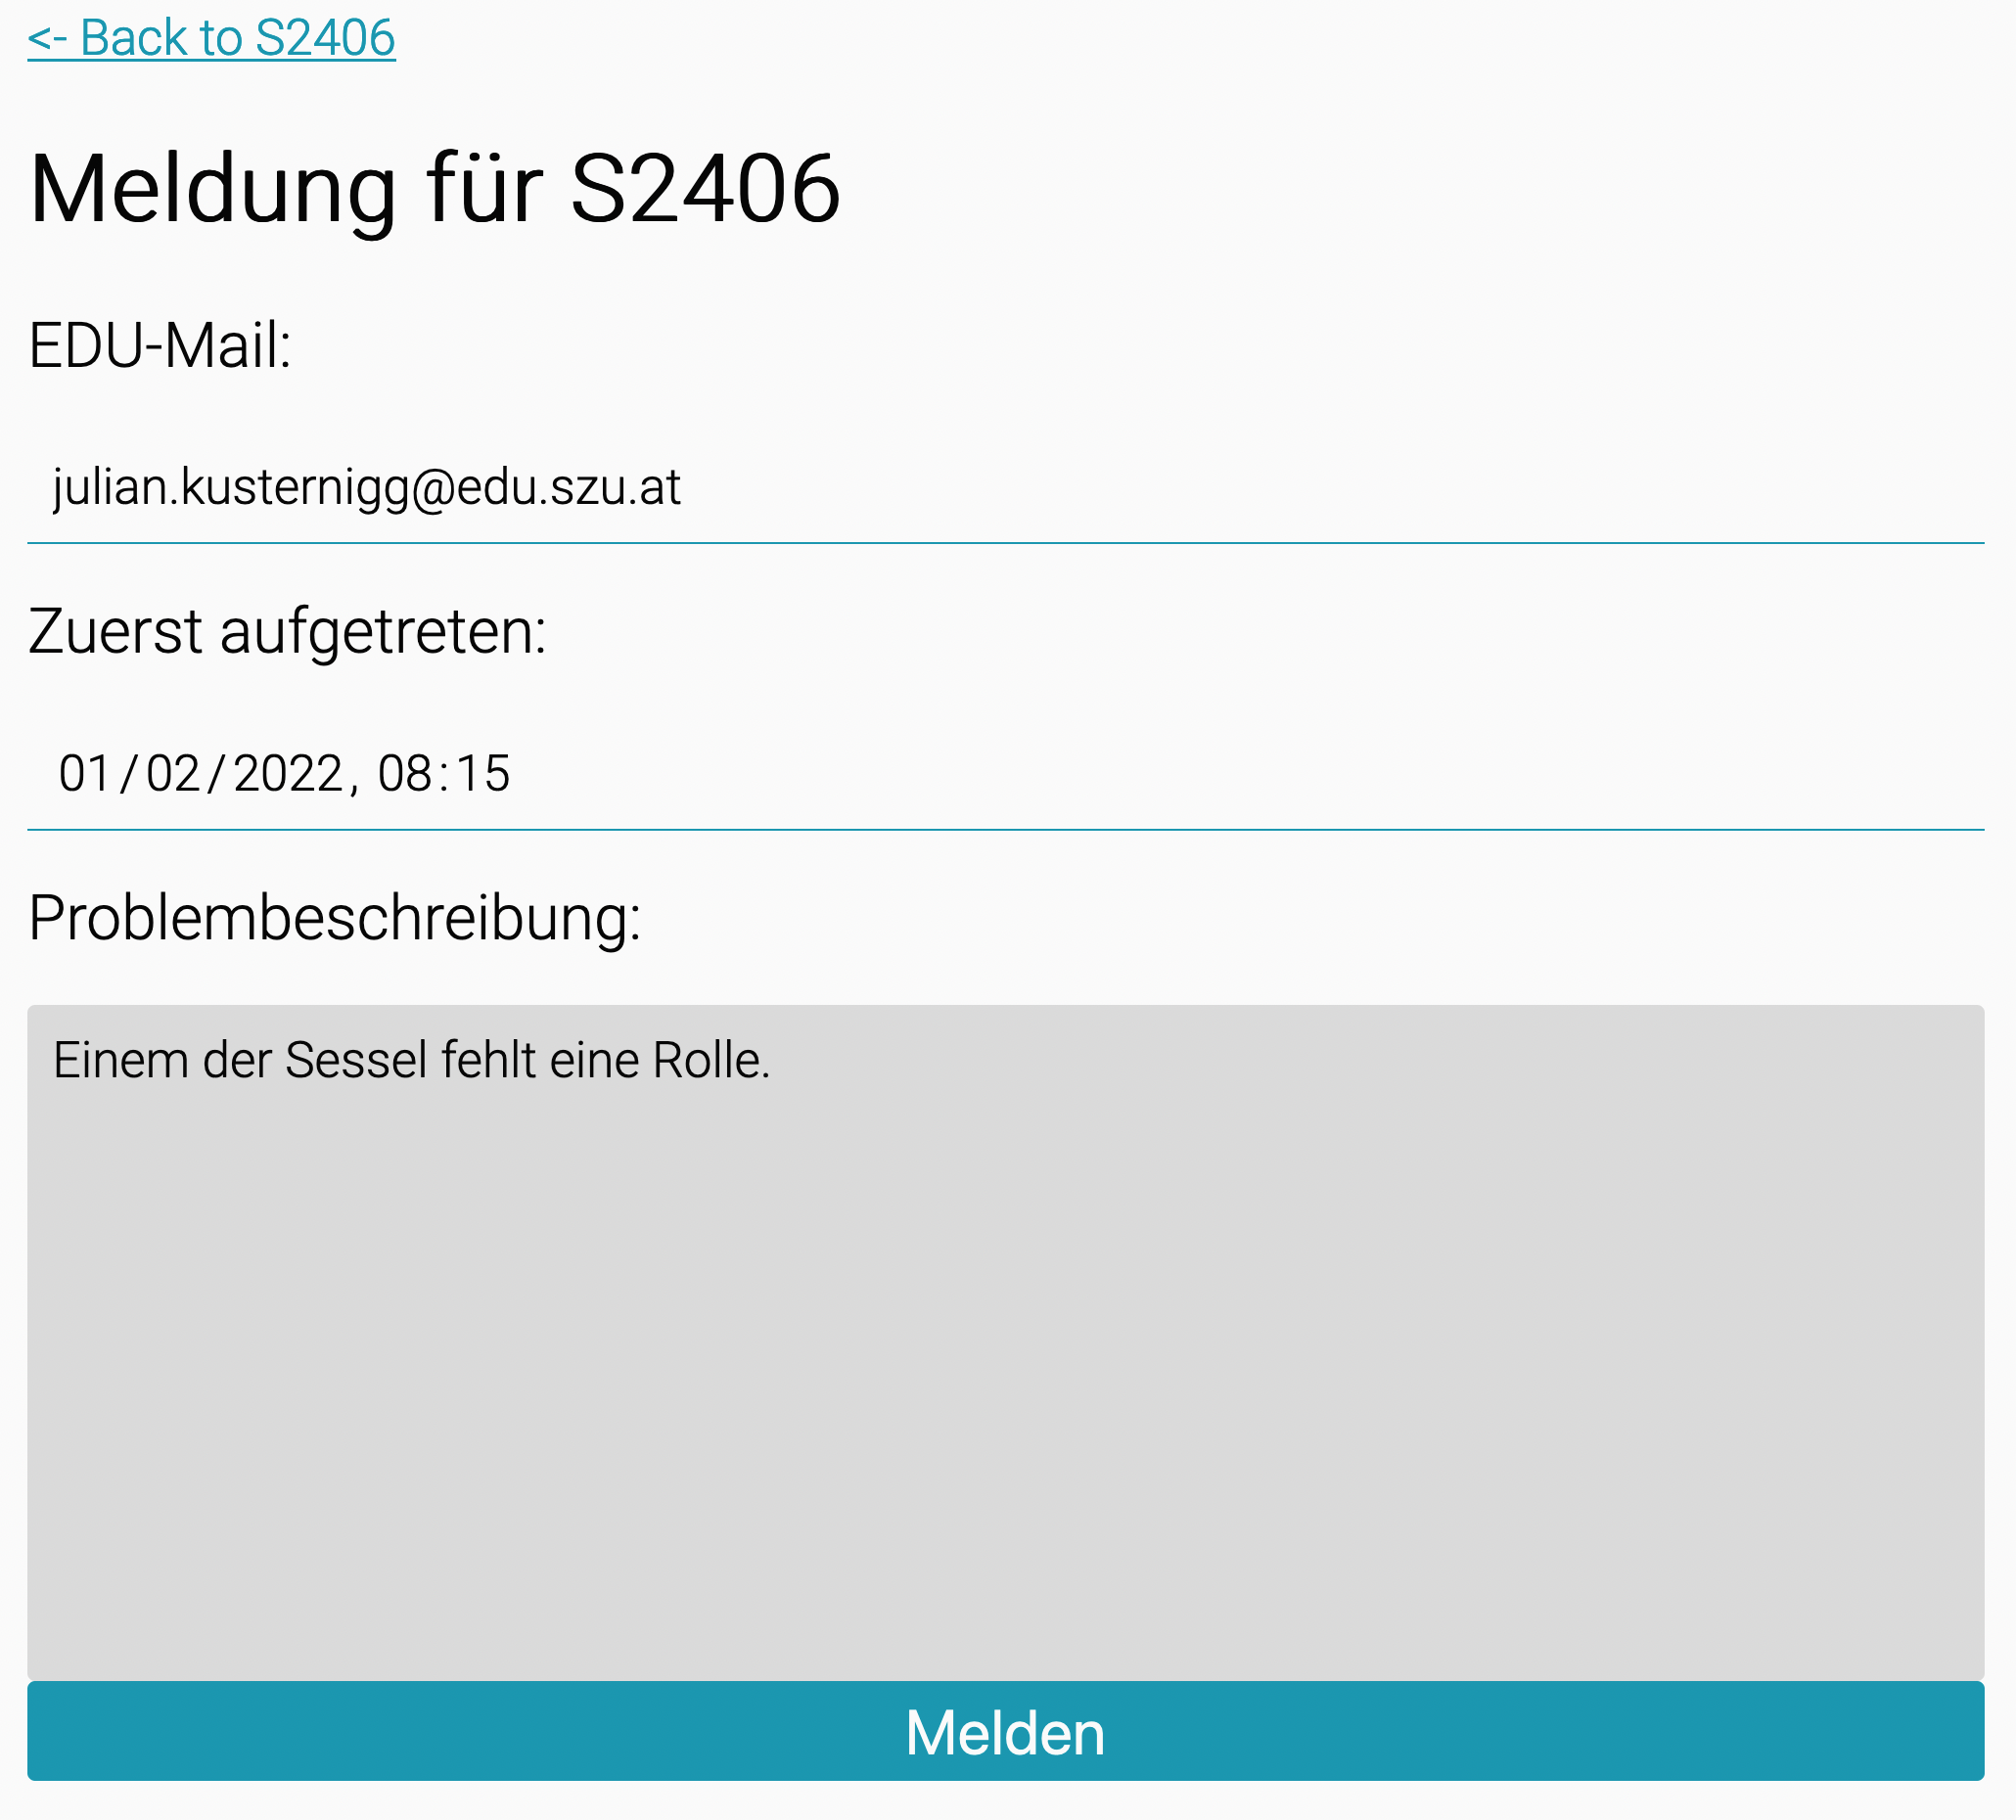
\includegraphics[width=120mm]{media/WebComponents/Meldungsseite_light.png}
    \caption{Meldungsseite}
\end{figure}

Eine Buchungsanfrage für einen Raum zu erstellen, geht ebenso einfach wie Defekte zu melden. Hierfür gibt man drei Dinge an: 
\begin{itemize}
    \item Den Tag, an dem man den Raum verwenden will
    \item Die Unterrichtsstunde, in der man startet
    \item Die Anzahl an Stunden, die man den Raum nutzen möchte
\end{itemize} 
Wie beim Melden gibt man auch hier eine EDU-Mailadresse an. Zusätzlich sollte man noch einen Buchungsgrund angeben, um kurz zu beschreiben wofür man den Raum benötigt.

\begin{figure}[H]
    \centering
    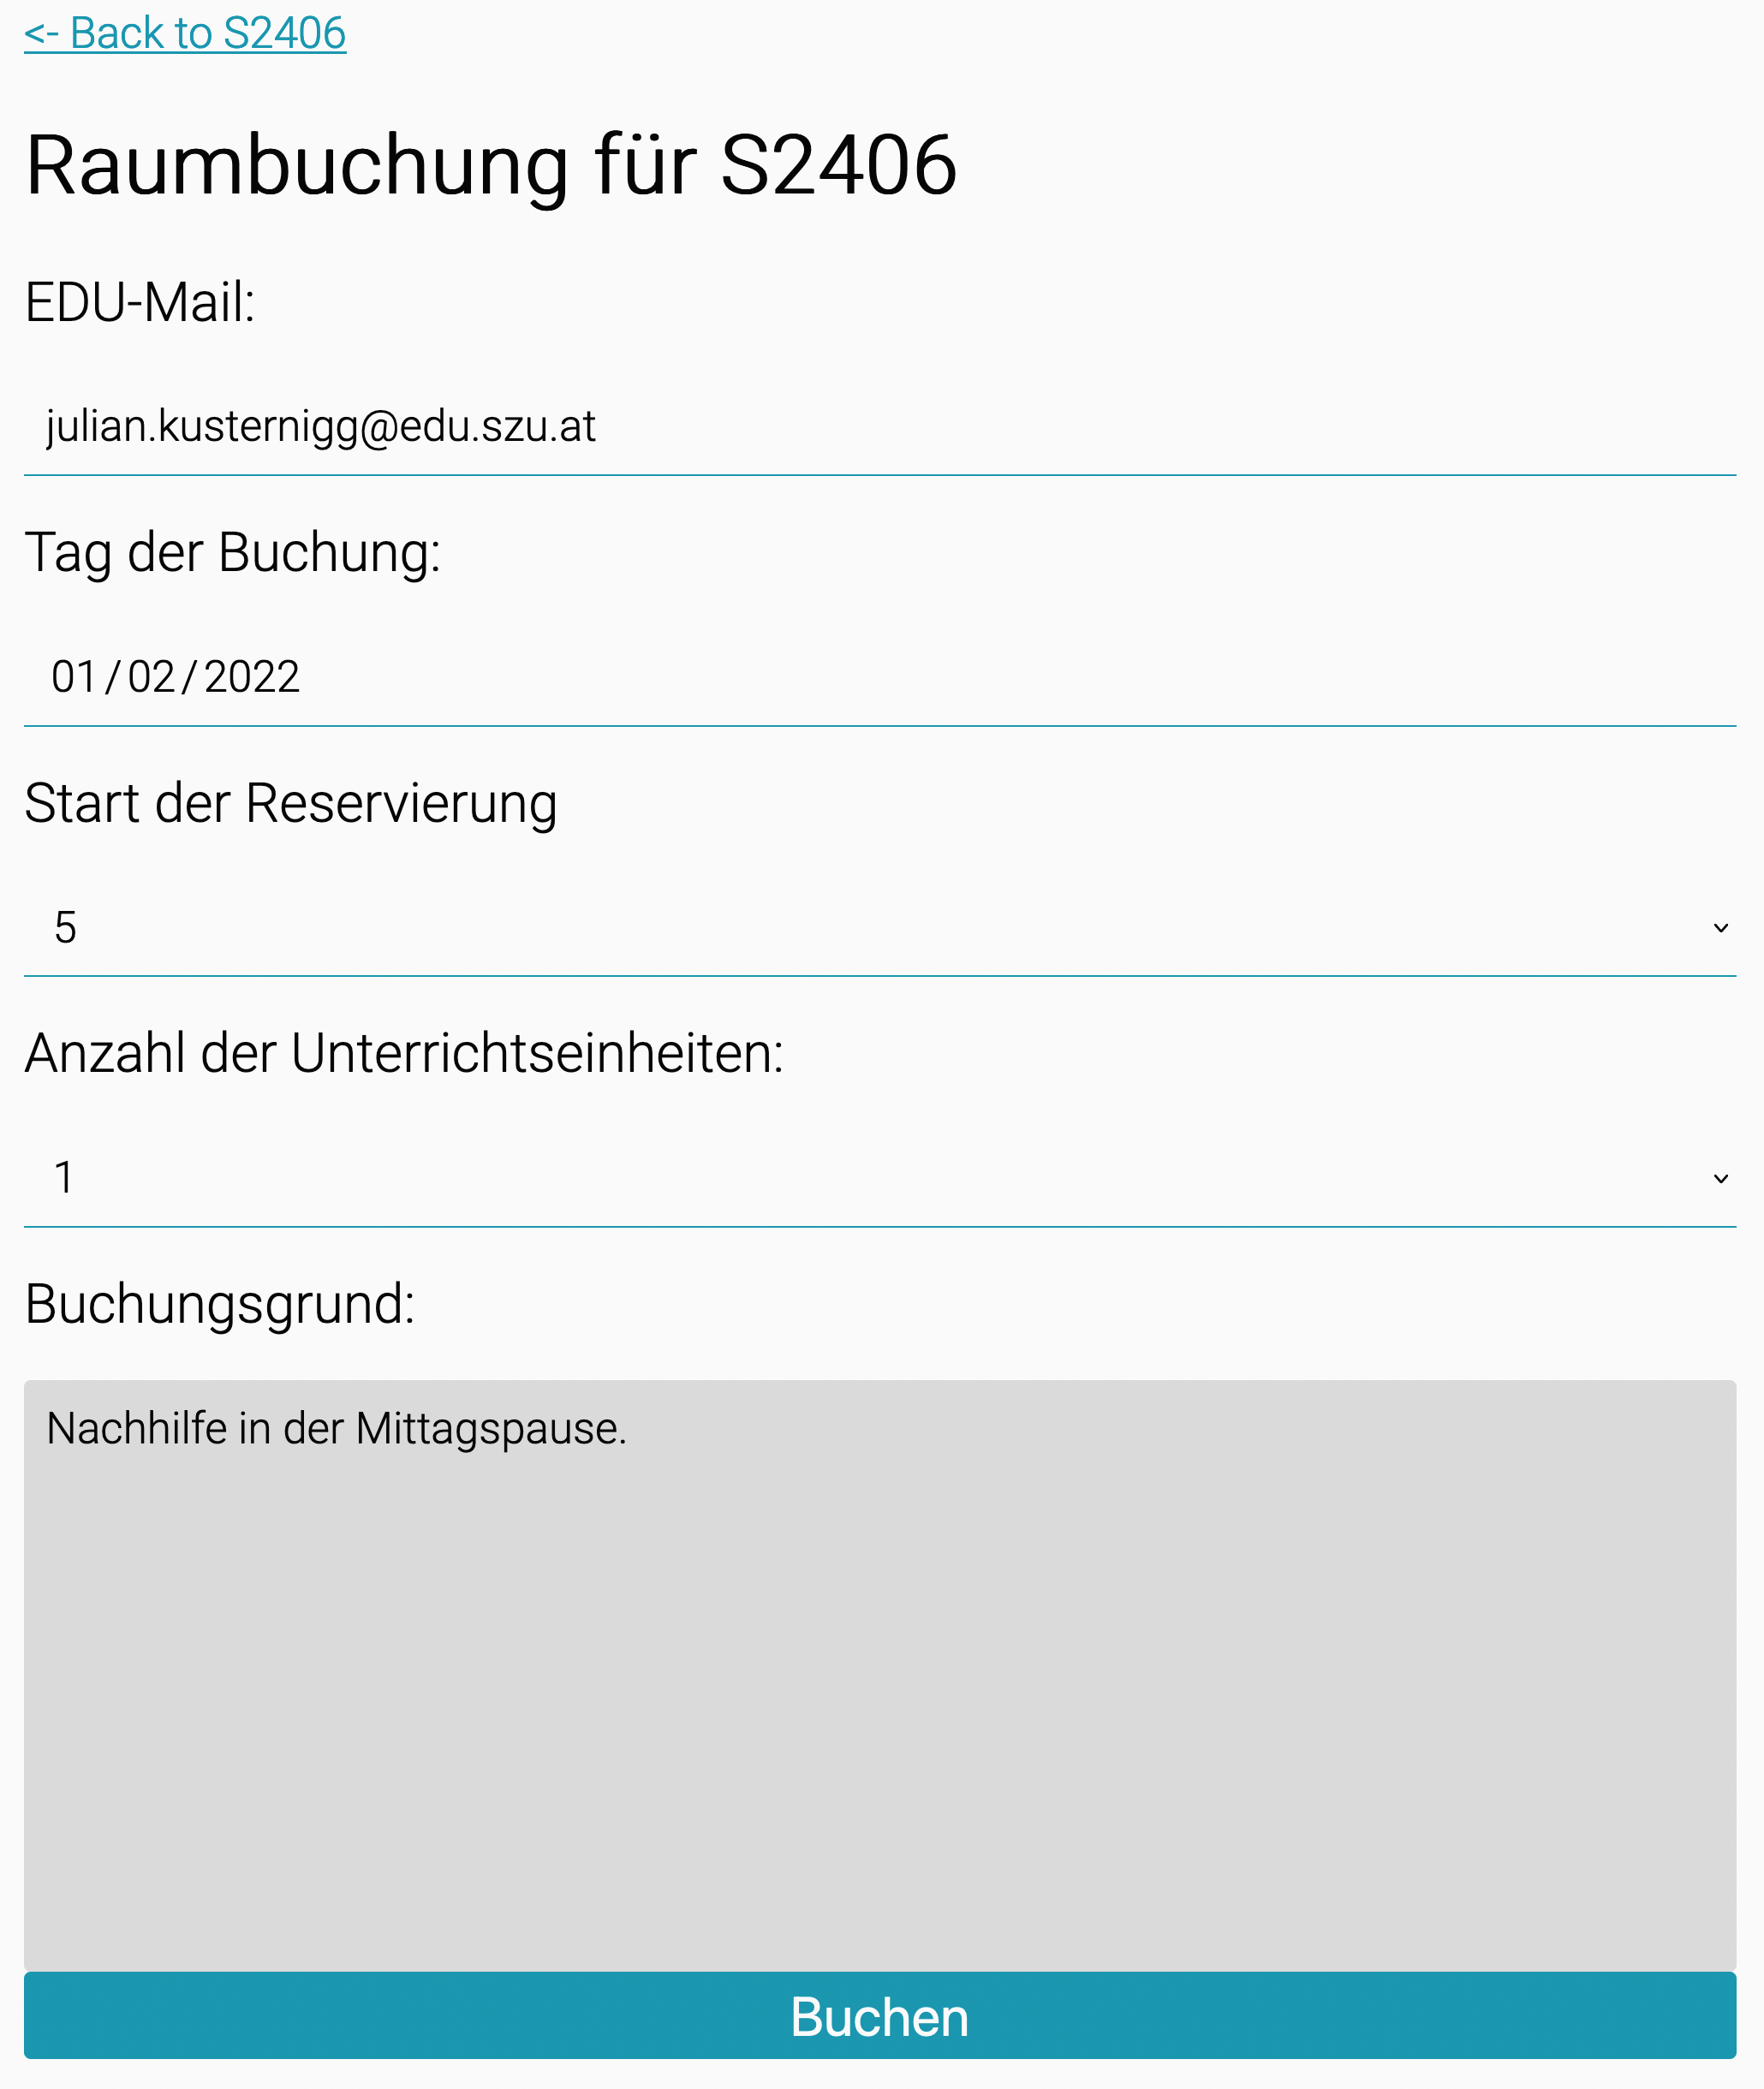
\includegraphics[width=120mm]{media/WebComponents/Buchungsseite_light.png}
    \caption{Buchungsseite}
\end{figure}


\hfive{"Admin Login" und "Dashboard"}
\label{sec:webcomplogdash}

Meldungen und Buchungen kann man im sogenannten "Admin Dashboard" einsehen. Damit nicht jeder die Raumbuchungen und Defektmeldungen sieht, muss man sich mit einem Administratorbenutzer anmelden. Jede Buchung und Meldung ist einem Administratorbenutzer zugeteilt und kann somit von diesem abgearbeitet werden. Im Fall von \ZELIA\ im Schulzentrum Ungargasse, sind diese Administratoren meist Abteilungsleiter*innen oder Lehrer*innen.

Wie schon beschrieben, muss man als Administrator angemeldet sein, um Zugriff auf alle Meldungen und Buchungen zu haben. Hierfür gibt es die "Admin Login"-Seite, welche über den normalen \ZELIA-Webserver aufgerufen werden kann. Auf dieser Webseite findet man eine Komponente, die ein Anmeldeformular anzeigt. Beim Anmelden wird die Anfrage an den Server geschickt und auf die Antwort gewartet. Wenn der Server mit einem "JSON-Web-Token" (siehe Kapitel Authentifizierung "JSON Web Token -- JWT" \ref{sec:jwt}) antwortet, wird dieser im "session storage" (siehe Kapitel "Webspeicher" \ref{sec:webstorage}) gespeichert und man wird auf die Übersichtsseite weitergeleitet.

\begin{figure}[H]
    \centering
    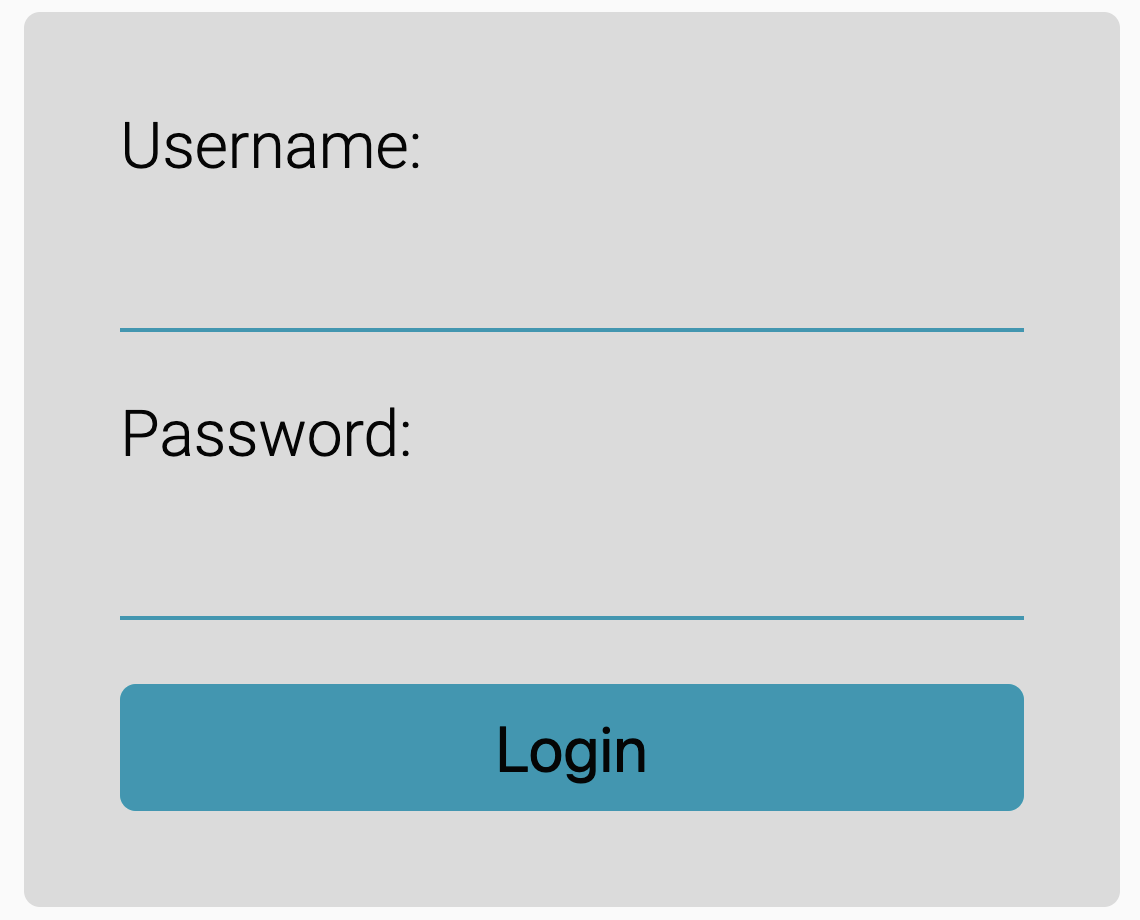
\includegraphics[width=120mm]{media/WebComponents/Login_light.png}
    \caption{Anmeldeseite}
\end{figure}

Landet man auf der "Admin Dashboard"-Seite, wird zuerst überprüft, ob ein Token im "session storage" gespeichert ist. Wenn keiner vorhanden ist, wird man sofort auf die Anmeldeseite umgeleitet. Bei einem vorhandenen Token werden alle Meldungen und Buchungen, die den Filtereinstellungen entsprechen, vom Server abgefragt. In dieser Anfrage wird auch der Token mitgeschickt. Am Server wird geprüft ob der Token gültig ist und wenn dies der Fall ist, bekommt der Client die angefragten Daten. Ist der Token ungültig, schickt der Server dem Client den HTTP-Code 401 "Unauthorized" und man wird zurück auf die Anmeldeseite umgeleitet.

Hat der Client die Buchungen und Meldungen erhalten, werden zwei Komponenten verwendet, um diese anzuzeigen. Anders als auf den anderen Seiten werden mehrere Instanzen dieser beiden Komponenten erstellt, um alle Daten darzustellen. Jede Buchung und Meldung ist somit in einer eigenen Instanz einer Komponente untergebracht. Beide dieser Komponenten können aufgeklappt werden, um alle damit verknüpften Informationen zu sehen. Zugeklappt bestehen sie aus einer Zusammenfassung der Daten (siehe Abbildung \ref{fig:admindashboard}).

Die Buchungskomponente hat zwei verschiedene Knöpfe, um die Buchungsanfrage zu verarbeiten. Einen zum "Akzeptieren" und den anderen zum "Ablehnen". Zusätzlich kann man einen kurzen Informationstext schreiben, der den Buchenden mit der Buchungsbestätigung gesendet wird. 

Die Komponente, welche Meldungen anzeigt, hat nur einen Knopf, um den Status der Meldung auf "geschlossen" zu setzen. Im Hintergrund gäbe es mehrere Auswahlmöglichkeiten eines Status, welche nicht im Frontend implementiert sind.

\begin{figure}[H]
    \centering
    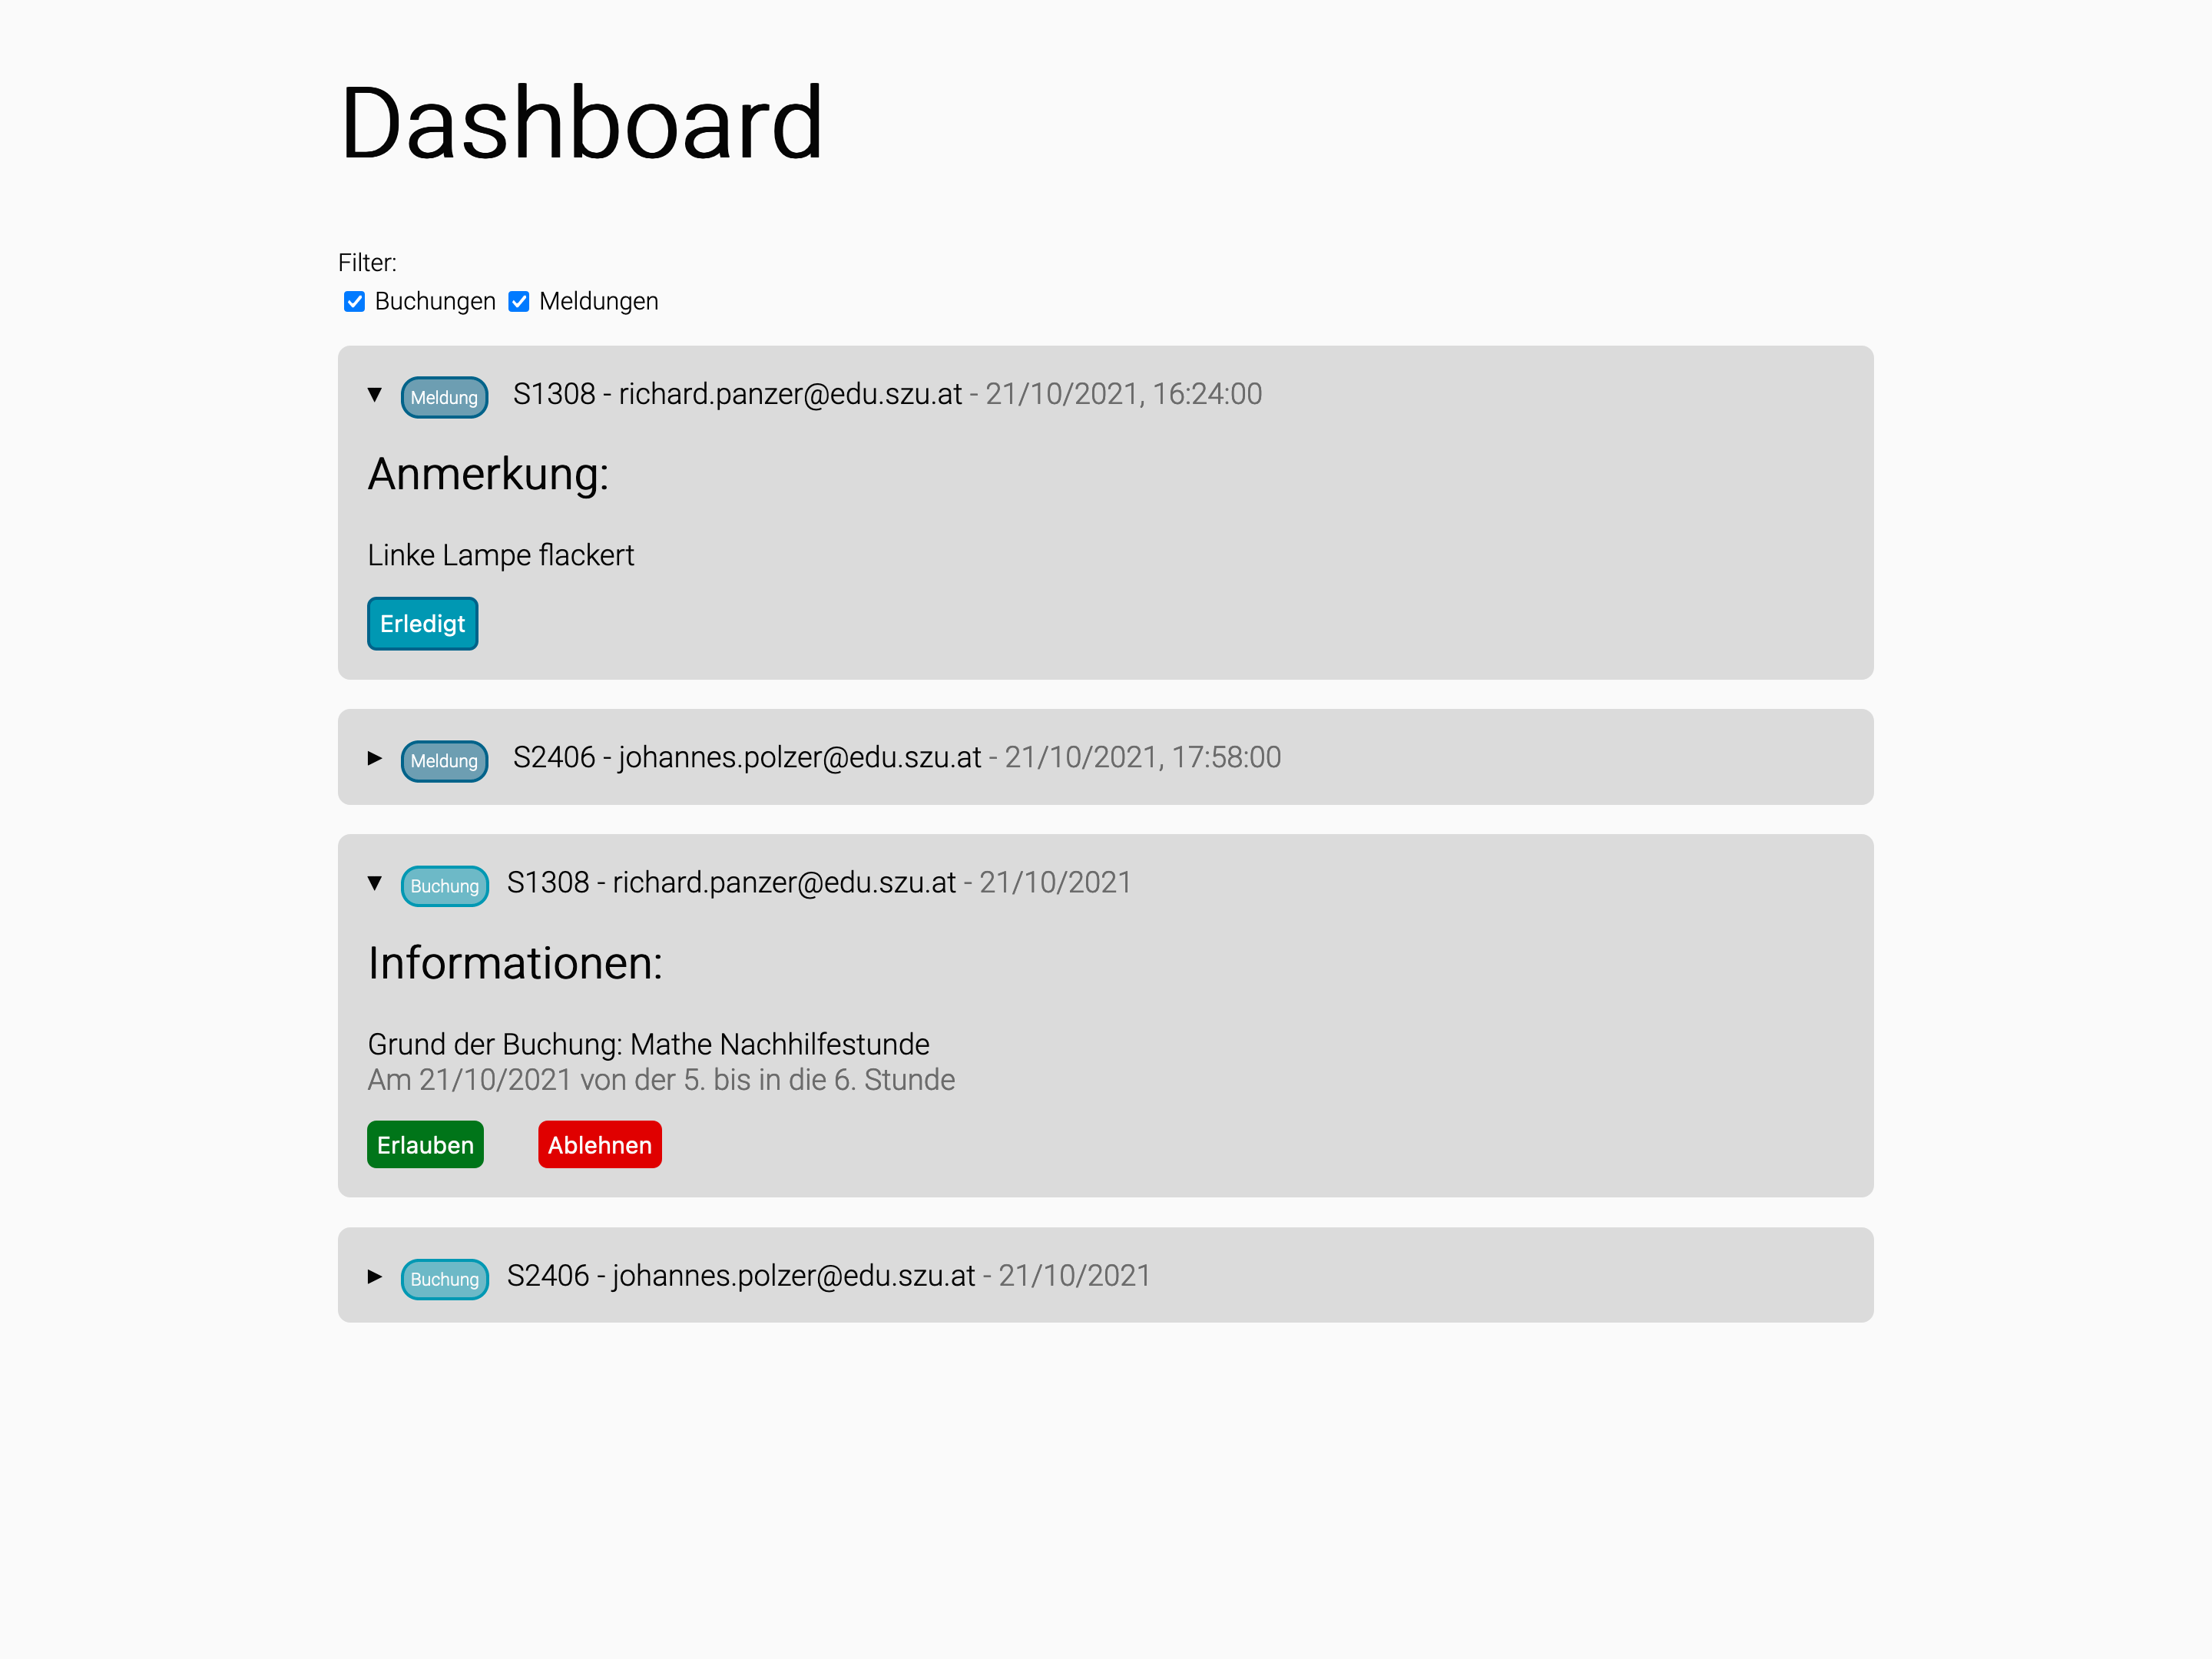
\includegraphics[width=120mm]{media/WebComponents/AdminSeite_light.png}
    \caption{Admin Dashboard}
    \label{fig:admindashboard}
\end{figure}

\begin{minipage}{\textwidth}
    \hfive{Die Fehlerseite}
    Die Fehlerseite ist keine eigene Seite mit einem fixierten Pfad, wie die anderen Seiten. Sie besteht nur aus der 404-"Not Found" Komponente und wird angezeigt, wenn auf einen nicht vorhandenen Pfad zugegriffen wird. 
\end{minipage}

So kommt \zb\ wenn der Pfad "{\ttfamily /admin/passwords}" aufgerufen wird:
    
\begin{figure}[H]
    \centering
    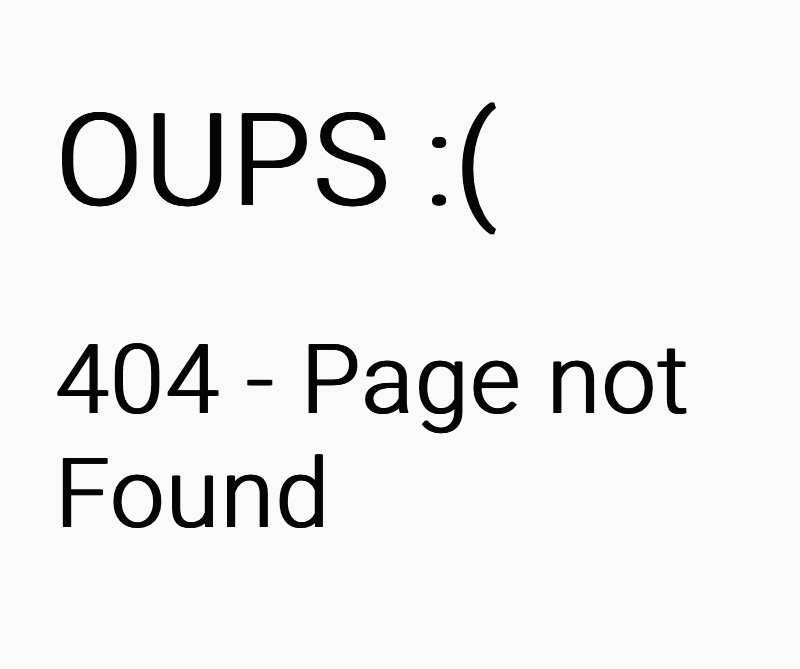
\includegraphics[width=80mm]{media/WebComponents/404.png}
    \caption{404 Fehler Seite}
\end{figure}